\documentclass[12pt,largemargins]{homework}
% \usepackage{subcaption}
% \usepackage{caption}
% \usepackage{float}
% \usepackage{listings}
% \usepackage{xcolor}
\usepackage{multirow}
\usepackage{array}

% TODO: replace these with your information
\newcommand{\hwname}{Ally Smith}
\newcommand{\hwemail}{Section A}
\newcommand{\hwtype}{Lab}
\newcommand{\hwnum}{1}
\newcommand{\hwclass}{}
\newcommand{\hwlecture}{0}
\newcommand{\hwsection}{Z}

\newcommand{\code}{\texttt}
\newcolumntype{M}{>{\centering\arraybackslash}m{4cm}}
\newcolumntype{S}{>{\centering\arraybackslash}m{4cm}}

\begin{document}
\maketitle

\question*{Generating Message Digest and MAC}
The easiest thing to notice after generating the different values was that
they vary in size. MD5 was 32 digits, or 128 bits. SHA-1 was 40 digits, or
160 bits. SHA-256 was 64 digits, or 256 bits. Other than that, there was no
discernable pattern in the hash values.

\question*{Keyed Hash and HMAC}
It is not necessary to use a key of a fixed size for HMAC.\@ This is because the
main calculation in an HMAC is provided by any cryptographic hash function,
which can take any input size and produce the same output size.

\question*{The Randomness of One-way Hash}
\begin{alphaparts}
    \questionpart{Input file contents:}
    \\\code{Lorem ipsum dolor sit amet, consectetur adipiscing elit,
    \\sed do eiusmod tempor incididunt ut labore et dolore
    \\magna aliqua.}

    \textbf{Hash Results:}
    \begin{center}
    % MD5
    % H1: e9faddf4d13ff1329e75e2573b86769b
    % H2: 5ac810b7288958194ad3282cfbfc4d8c
    % SHA256
    % H1: dfee893b95f63da38bd4a2e50826bc11cc9c5b90c7db14ec1a5ce83db1e90fea
    % H2: 2cc68a94df19e743036d5c3f8f88618ef2da49e0c5ac809ac5111ce584e453e6
    \begin{tabular}{|c|M|S|}\hline
        \textbf{Hash} & \textbf{MD5} & \textbf{SHA256} \\\hline
        $H_1$ & \code{e9faddf4d13ff132 9e75e2573b86769b} & \code{dfee893b95f63da3
        8bd4a2e50826bc11 cc9c5b90c7db14ec 1a5ce83db1e90fea}\\\hline
        $H_2$ & \code{5ac810b728895819 4ad3282cfbfc4d8c} & \code{2cc68a94df19e743
        036d5c3f8f88618e f2da49e0c5ac809a c5111ce584e453e6}\\\hline
        Shared bits & 59 of 128 & 121 of 256 \\\hline
    \end{tabular}
    \end{center}
\end{alphaparts}

\section*{Appendix}
The script used to count shared bits between $H_1$ and $H_2$ for question 3:
\begin{center}
    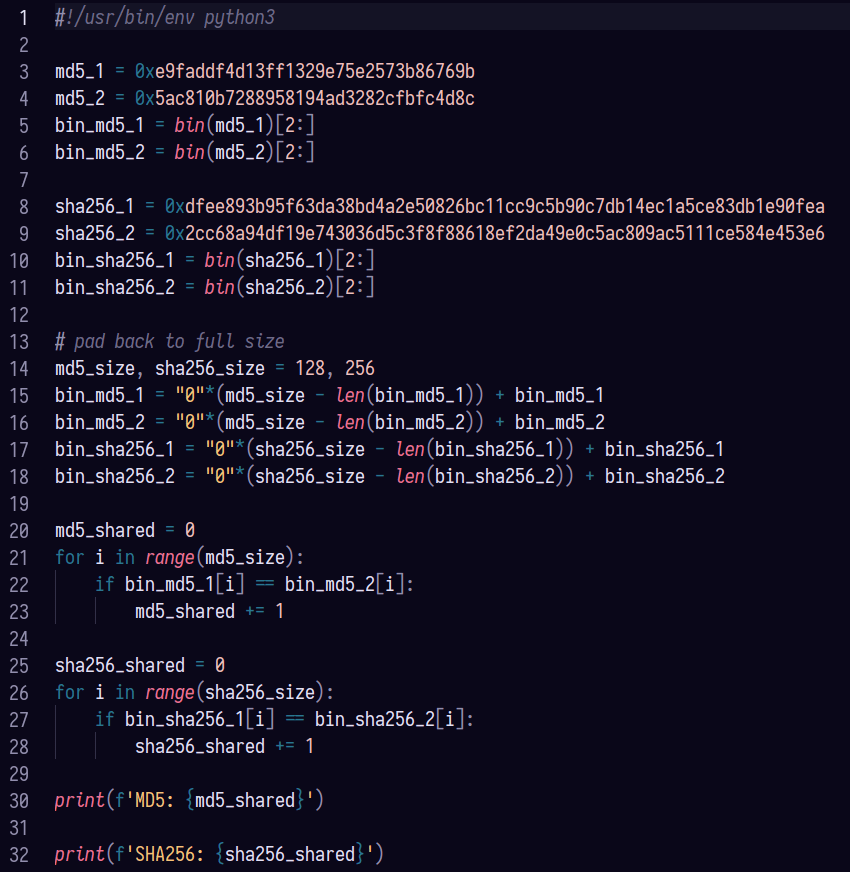
\includegraphics[width=.75\textwidth]{count-shared-bits-py.png}
\end{center}

\end{document}